\documentclass[11pt]{article}

\usepackage{fix-cm}
\usepackage{tikz}
\usepackage{forest} 
\usepackage{amsmath,amsthm} 
\usepackage{amssymb}
\usepackage[framemethod=tikz]{mdframed}
% \usepackage{draculatheme}
\usepackage{mathrsfs}
\usepackage{changepage}
\usepackage{multicol}
\usepackage{mathtools}
\usepackage{hyperref}
\usepackage{slashed}
\usepackage{enumerate}
\usepackage{booktabs}
\usepackage{enumitem}
\usepackage{kantlipsum} 
\usepackage{tabularx}
\usepackage{array}
\usepackage{makecell}
\usepackage{pgfplots}
\pgfplotsset{compat=1.18}
\usetikzlibrary{
	decorations.markings,
	trees,
	arrows,
	automata,
	shapes,
	backgrounds,
	calc,
	patterns
}

\setlength{\parindent}{0pt}

\newmdenv[
	topline=false,
	bottomline=true,
	rightline=false,
	leftline=true,
	linewidth=1.5pt,
	linecolor=black, % default color, will be overridden in custom commands
	% backgroundcolor=draculabg, % Needed for Dracula theme
	% fontcolor=draculafg, % Needed for Dracula theme
	innertopmargin=0pt,
	innerbottommargin=5pt,
	innerrightmargin=10pt,
	innerleftmargin=10pt,
	leftmargin=0pt,
	rightmargin=0pt,
	skipabove=\topsep,
	skipbelow=\topsep,
]{customframedproof}

\newenvironment{proofpart}[2][black]{
    \begin{mdframed}[
        topline=false,
        bottomline=false,
        rightline=false,
        leftline=true,
        linewidth=1pt,
        linecolor=#1!40, % Custom color
        innertopmargin=10pt,
        innerbottommargin=10pt,
        innerleftmargin=10pt,
        innerrightmargin=10pt,
        leftmargin=0pt,
        rightmargin=0pt,
        % skipabove=\topsep,
        % skipbelow=\topsep%
    ]
    \noindent
    \begin{minipage}[t]{0.08\textwidth}%
        \textbf{#2}%
    \end{minipage}%
    \begin{minipage}[t]{0.90\textwidth}%
        \begin{adjustwidth}{0pt}{0pt}%
}{
    \end{adjustwidth}
    \end{minipage}
    \end{mdframed}
}

\newenvironment{solution}
  {\textit{Solution.}}



%%% AESTHETICS %%%
%-%-%-%-%-%-%-%-%-%-%-%-%-%-%-%-%-%-%-%-%-%-%-%-%-%-%-%-%-%-%-%-%-%-%-%-%-%-%


%%% Dimensions and Spacing %%%
\usepackage[left=0.5in,right=0.5in,top=1in,bottom=1in]{geometry}
% \usepackage{setspace}
% \linespread{1}
\usepackage{listings}

%%% Define new colors %%%
\usepackage{xcolor}
\definecolor{orangehdx}{rgb}{0.96, 0.51, 0.16}

% Normal colors
\definecolor{xred}{HTML}{BD4242}
\definecolor{xblue}{HTML}{4268BD}
\definecolor{xgreen}{HTML}{52B256}
\definecolor{xpurple}{HTML}{7F52B2}
\definecolor{xorange}{HTML}{FD9337}
\definecolor{xdotted}{HTML}{999999}
\definecolor{xgray}{HTML}{777777}
\definecolor{xcyan}{HTML}{80F5DC}
\definecolor{xpink}{HTML}{F690EA}
\definecolor{xgrayblue}{HTML}{49B095}
\definecolor{xgraycyan}{HTML}{5AA1B9}

% Dark colors
\colorlet{xdarkred}{red!85!black}
\colorlet{xdarkblue}{xblue!85!black}
\colorlet{xdarkgreen}{xgreen!85!black}
\colorlet{xdarkpurple}{xpurple!85!black}
\colorlet{xdarkorange}{xorange!85!black}
\definecolor{xdarkcyan}{HTML}{008B8B}
\colorlet{xdarkgray}{xgray!85!black}

% Very dark colors
\colorlet{xverydarkblue}{xblue!50!black}

% Document-specific colors
\colorlet{normaltextcolor}{black}
\colorlet{figtextcolor}{xblue}

% Enumerated colors
\colorlet{xcol0}{black}
\colorlet{xcol1}{xred}
\colorlet{xcol2}{xblue}
\colorlet{xcol3}{xgreen}
\colorlet{xcol4}{xpurple}
\colorlet{xcol5}{xorange}
\colorlet{xcol6}{xcyan}
\colorlet{xcol7}{xpink!75!black}

% Blue-Purple (should just used colorbrewer...)
\definecolor{xrainbow0}{HTML}{e41a1c}
\definecolor{xrainbow1}{HTML}{a24057}
\definecolor{xrainbow2}{HTML}{606692}
\definecolor{xrainbow3}{HTML}{3a85a8}
\definecolor{xrainbow4}{HTML}{42977e}
\definecolor{xrainbow5}{HTML}{4aaa54}
\definecolor{xrainbow6}{HTML}{629363}
\definecolor{xrainbow7}{HTML}{7e6e85}
\definecolor{xrainbow8}{HTML}{9c509b}
\definecolor{xrainbow9}{HTML}{c4625d}
\definecolor{xrainbow10}{HTML}{eb751f}
\definecolor{xrainbow11}{HTML}{ff9709}

%%% FIGURES %%%
\usepackage{graphicx}  
% \graphicspath{ {images/} }  
% \numberwithin{figure}{section}
\usepackage{float}
\usepackage{caption}

%%% Hyperlinks %%%
\usepackage{hyperref}
\definecolor{horange}{HTML}{f58026}
\hypersetup{
	colorlinks=true,
	linkcolor=horange,
	filecolor=horange,      
	urlcolor=horange,
}

\newcommand{\mysqrt}[1]{%
  \mathpalette\foo{#1}%
}
\newcommand{\dmysqrt}[1]{%
  \mathpalette\foodisplay{#1}%
}

\newcommand{\sol}[1]{
    \begin{customframedproof}[linecolor=orangehdx!75,]
        \begin{solution}
        #1
        \end{solution}
    \end{customframedproof}
}

% !TeX spellcheck = off
\newcommand{\foo}[2]{%
	% #1: math style, #2: content
	\sbox0{\(#1\sqrt{#2}\)}% Measure the size of the standard sqrt in the current style
	\begin{tikzpicture}[baseline=(sqrt.base)]
    	\node[inner sep=0, outer sep=0] (sqrt) {\(#1\sqrt{#2}\)}; % Use the current math style
    	\draw([yshift=-0.045em]sqrt.north east) -- ++(0,-0.5ex); % Draw the tick
  	\end{tikzpicture}%
}
% !TeX spellcheck = off
\newcommand{\foodisplay}[2]{%
    % #1: math style, #2: content
    \sbox0{\(#1\sqrt{#2}\)}% Measure the size of the standard sqrt in the current style
    \begin{tikzpicture}[baseline=(sqrt.base)]
		\node[inner sep=0, outer sep=0] (sqrt) {\(\displaystyle\sqrt{#2}\)}; % Force displaystyle
    	\draw[line width=0.4pt] ([yshift=-0.044em]sqrt.north east) -- ++(0,-0.5ex); % Draw the tick
	\end{tikzpicture}%
}

\newcommand{\barNotationT}[1]{\bigg|_{t = #1}}

\newcommand{\cyanit}[1]{\textit{\textcolor{cyan}{#1}}}

\newcommand{\brackett}[1]{\left\langle #1 \right\rangle}

\newcommand{\norm}[1]{\left\lVert \mathbf{#1}\right\rVert}

\newcommand{\imb}{\mb{i}}
\newcommand{\jmb}{\mb{j}}
\newcommand{\kmb}{\mb{k}}
\newcommand{\rmb}{\mb{r}}
\newcommand{\umb}{\mb{u}}

\newcommand{\vecfuc}[2]{\mb{#1}(#2)}
\newcommand{\dvecfuc}[2]{\mb{#1}'(#2)}
\newcommand{\normdvecfuc}[2]{||\mb{#1}'(#2)||}

\newcommand{\proj}{\text{proj}}

\newcommand{\mb}[1]{\mathbf{#1}}

% \renewcommand{\theenumi}{\arabic{enumi}} 
% \renewcommand{\labelenumi}{\theenumi.}

\title{Probability and Statistics: Practice Set 4}
\author{Paul Beggs}
\date{\today}

%%% Custom Comands %%%
% Natural Numbers 
\newcommand{\N}{\ensuremath{\mathbb{N}}}

% Whole Numbers
\newcommand{\W}{\ensuremath{\mathbb{W}}}

% Integers
\newcommand{\Z}{\ensuremath{\mathbb{Z}}}

% Rational Numbers
\newcommand{\Q}{\ensuremath{\mathbb{Q}}}

% Real Numbers
\newcommand{\R}{\ensuremath{\mathbb{R}}}

% Complex Numbers
\newcommand{\C}{\ensuremath{\mathbb{C}}}

\newcommand{\I}{\ensuremath{\mathbb{I}}}

\newcommand{\p}{\partial}

\newcommand{\mbi}{\mathbf{i}}
\newcommand{\mbj}{\mathbf{j}}
\newcommand{\mbk}{\mathbf{k}}
\newcommand{\mbr}{\mathbf{r}}

\newcommand{\bigpfrac}[2]{\left( \frac{#1}{#2} \right)}
\newcommand{\negbigpfrac}[2]{\left(- \frac{#1}{#2} \right)}


\begin{document}

\maketitle

\begin{enumerate}
    \item (2 points) A device that continuously measures and records seismic activity is placed in a remote region. The time, \(T\), to failure of this device is exponentially distributed with mean 3 years. Since the device will not be monitored during its first two years of service, the time to discovery of its failure is \(X = \max(T,2)\). Find \(E(X)\). You may approximate any integrals using your calculator.
    \sol{

    }
    \item (1 point each) An actuary determines that the annual number of tornadoes in counties \(P\) and \(Q\) are jointly distributed as follows: \\
    \begin{tabular}{r||r|r|r|r}
        & \multicolumn{4}{c}{County \(Q\)} \\
        County \(P\) & 0 & 1 & 2 & 3 \\ \hline\hline
        0 & 0.12 & 0.06 & 0.05 & 0.02 \\ 
        1 & 0.13 & 0.15 & 0.12 & 0.03 \\
        2 & 0.05 & 0.15 & 0.10 & 0.02
    \end{tabular}
    \begin{enumerate}
        \item Determine the conditional expected number of tornados in county \(Q\), given that there are no tornados in county \(P\).
        \sol{

        }
        \item Calculate the conditional variance of the annual number of tornadoes in county \(Q\), given that there are no tornadoes in county \(P\).
        \sol{

        }
    \end{enumerate}
    \item Let \(X\) and \(Y\) be random variables with joint pmf \(f(x, y) = c  (xy^2 + x)\), where \(x = 1, 2, 3\) and \(|y - 3| + x = 0, 1, 2, 3\).
    \begin{enumerate}
        \item (2 point) Explicitly list the 9 points which are in the support (i.e. the sample space):
        \sol{

        }
        \item (1 point) Determine a value of c that makes this a pmf.
        \sol{

        }
        \item (1 point) On the axes given, show the sample space, the individual probabilities, and the marginal pmfs.
        \sol{
            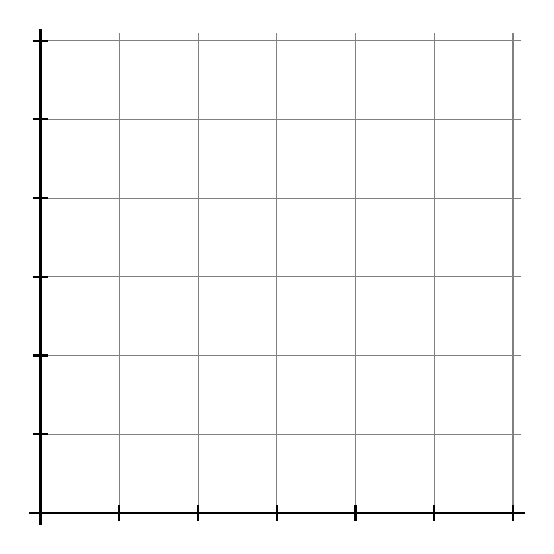
\begin{tikzpicture}
                \draw[step=1cm, gray, thin] (0,0) grid (6,6);
                \draw[step=1cm, gray, thin] (-.1,-.1) grid (6.1,6.1);
                \draw[step=1cm, black, thick] (-.1,-.1) grid (6, 0.1);
                \draw[step=1cm, black, thick] (-.1,-.1) grid (0.1, 6);
                \draw[step=1cm, black, thick] (-.15,0) to (6.15,0);
                \draw[step=1cm, black, thick] (0,-0.15) to (0,6.15);
            \end{tikzpicture}
        }
        \item (2 points) Find each of \(\mu_{X}\) and \(\mu_{Y}\).
        \sol{

        }
        \item (2 points) find each of \(\sigma^{2}_{X}\) and \(\sigma^{2}_{Y}\). 
        \sol{

        }
        \item (2 points) Find each of \(\text{Cov}(X,Y)\) and \(\rho\).
        \sol{

        }
        \item (1 point) Find the equation of the least squares regression line.
        \sol{

        }
    \end{enumerate}
    \item Let \(X\) and \(Y\) be continuous random variables with joint pdf \(f(x,y) = kxy^{2}\), for \(0 \le x \le 1\) and \(0 \le y \le x^{2}\), and some constant \(k\).
    \begin{enumerate}
        \item (1 point) On the axes given, show the sample space
        \sol{
            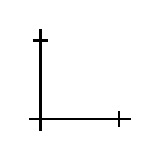
\begin{tikzpicture}
                \draw[step=1cm, black, thick] (-.1,-.1) grid (1, 0.1);
                \draw[step=1cm, black, thick] (-.1,-.1) grid (0.1, 1.1);
                \draw[step=1cm, black, thick] (-.15,0) to (1.15,0);
                \draw[step=1cm, black, thick] (0,-0.15) to (0,1.15);
            \end{tikzpicture}
        }
        \item (1 point) Find the value of \(k\) which makes this a pdf.
        \sol{

        }
        \item (2 points) Find each of \(f_{X}(x)\) and \(f_{Y}(y)\).
        \sol{
            
        }
        \item (2 points) Find each of \(\mu_{X}\) and \(\mu_{Y}\).
        \sol{
            
        }
        \item (2 points) Find each of \(\sigma_{X}^{2}\) and \(\sigma_{Y}^{2}\).
        \sol{
            
        }
        \item (2 points) Find each of \(\text{Cov}(X,Y)\) and \(\rho\).
        \sol{
            
        }
        \item (1 point) Are \(X\) and \(Y\) independent? Justify this answer.
        \sol{
            
        }
    \end{enumerate}
    \item (2 points each) (2 points each) Let \(X\) be the weight of robin eggs, in grams, and \(Y\) be the daily high temperature, in degrees Celsius. Assume that \(X\) and \(Y\) have a bivariate normal distribution with \(\mu_{X} = 145.2\), \(\sigma_{X}^{2} = 109.2\), \(\mu_{Y} = 23.5\), \(\sigma_{Y}^{2} = 21.8\), and \(\rho = -0.34\).
    \begin{enumerate}
        \item Find the probability that a robin egg weights between 142 and 152 grams.
        \sol{
            
        }
        \item Given that it has been a warm year, so that \(Y = 25.1\), find the probability that a robin egg weights between 142 and 152 grams.
        \sol{
            
        }
    \end{enumerate}
\end{enumerate}

\end{document} 